\section{System design}
In this section, the requirement and tasks are discussed. Over the past 12 months, we closely worked with two domain researchers; in urban air quality analysis and forecasting. One researcher \UC{(R1)} studies the atmospheric diffusion of air pollutants and the other researcher (R2) is working on air pollutant forecasts through machine learning techniques. Both of them have strong domain experience in air quality forecasting. 

\subsection{Analytical  Goals}
% We have distilled the following goals based on an informal interview with domain experts who work on utilizing RNN models to predict weather pollution. 

During the discussions, three general goals were distilled:. 

\begin{itemize}
  \item G1: Understand the RNN model behavior/mechanism in high-dimensional forecasts. 
  \item G2: Understand the feature importance. 
  \item G3: Support case-based exploration.
\end{itemize}

% \textbf{G1: Understand the RNN model behavior/mechanism in high-dimensional forecasts.} 
% Since the target users already have basic knowledge about the RNN models including their structure and theory, the crucial requirement to understand the model is to explain how such structure works for the forecasting tasks. 
% For example, how do the hidden units capture the information from the time-series data? 
% Understanding the hidden units is challenging because of the complicated many-to-many relationship which exists among hundreds of hidden units and features. 
% Compared with tasks related to natural language or image processing, it is difficult to extract semantic information from  high-dimensional time-series data. 
% An effective way to calculate, summarize, and visualize the relationship as well as the high-dimensional time-series data is required. 

% \textbf{G2: Understand the feature importance.} 
% Unlike R1, the feature importance explains the machine learning model by considering the model as a black box. 
% In general, the feature importance measures the contribution of features to the forecasting result and can be effectively understood by the end user who has rich domain knowledge. 
% In this discussion session, the domain experts are extremely interested in which features always have a large contribution to the output while some of the features influence the result only under specific conditions. 
% Understanding the feature importance reflected by deep learning models can increase the trust of the end users or allow the users to justify the result.  
% Existing techniques include back-propagation-based approaches and perturbation-based forward-propagation approaches. 
% However, most of these methods target calculating the feature importance/contribution at the individual level and fail to provide an overview across all the features.  

% \textbf{G3: Support case-based exploration.} 
% Case-based exploration is one of the most effective strategies for humans to interpret machine learning models. 
% It is based on the assumption that a new problem can be resolved by the solutions of previous similar problems, which can serve as a scaffold for understanding the challenges. 
% Adopting case-based exploration can facilitate users in obtaining an overview of RNN models such as observing which types of data the model tends to make errors or identifying the most critical features that can affect a prediction. 
% Users can compare two similar sequences to see if the model performance is consistent or examine the predictions at consecutive time steps to estimate when the model's behavior changes dramatically. 
% However, providing case-based exploration for RNN models is challenging as the system needs to flexible enough for users to filter and search the cases of interest. 
% To examine a case, which consists of high-dimensional vectors from multiple time steps, the system is also required to be scalable and able to provide informative memorization at the same time. 
% We aim to provide users a flexible and effective case-based exploration workflow.

\subsection{Design Tasks}
\label{section:design_tasks}
To fulfill the aforementioned design goals, we have distilled the following analytical tasks:

\textbf{T1: Encode hidden state statistics.}
Hidden states, a direct reflection of a model's intermediate results, are critical for revealing the information captured by a model (\textbf{G1, G2}).
Visualizing hidden state statistics can provide a holistic picture of a model's capacity and behavior.
% For example, summarizing the overall activeness of all the hidden units can help users estimate whether the current parameter size is appropriate.
By linking the hidden state activeness with data and prediction results, users can also identify the blind points where models tend to predict incorrectly.
Thus, our system should support encoding various hidden state statistics such as value distribution and the data coverage.

\textbf{T2: Measure and encode feature importance across multiple scales.}
The appropriate technique should be embedded in the system to measure feature importance. 
Also, the visual analytics system should allow users to explore feature importance at different scales. 
For example, the overview level ranks and presents feature importance summarized from the whole dataset. 
The group level exploration enables users to select a subset of cases and explore the feature importance distribution, while the individual level will focus on the feature importance of the single case.


\textbf{T3: Analyze the response between features and hidden states.}
Measuring the correlation relationship between features and hidden states is the key factor in revealing what patterns are captured by the model (\textbf{G1}). 
By inspecting what features can activate certain hidden units, users can know how the model pays attention to different factors. 
This also enables users to see if the model has utilized all the features or only focus on the most important ones. 
In addition, targeting at the complicated many-to-many relationship, the hidden states as well as the features should be clustered to alleviate the burden on end users. 


\textbf{T4: Support temporal analysis.}
One major advantage of RNNs is that they can capture time-dependent sequence information.
The prediction is affected not only by the features from the last time step, but also the historical information being passed along the sequence.
Showing what information is preserved along the sequence and what information is discarded helps users better understand how the temporal information is utilized by the model.
In addition, users can identify the most critical time step that causes a dramatic change in the model's prediction.
For these reasons, the system should be able to support temporal analysis when interpreting the model's behaviors.


\textbf{T5: Identify data clusters and outliers.}
To support case-based reasoning, users need to first obtain a data overview by identifying the data clusters and outliers (\textbf{G1, G3}).
This provides concrete examples to guide users in further exploring the data of interests.
For example, users can estimate how many categories of data share the same or similar prediction results by observing data clusters.
Users can also inspect the outliers that have distinct prediction results to detect if the model behaves incorrectly according to certain domain knowledge.
We aim to provide users an overview of the data and enable them to compare different data and their resulting predictions.

\textbf{T6: Enable case comparison.}
As the key concept of case-based exploration is to use existing knowledge to solve similar new problems, enabling sequence comparison is necessary for interpreting RNN models (\textbf{R1}). 
Many scenarios require users to compare the prediction processes of multiple sequences at the same time.
For example, users may need to examine two similar but slightly different sequences to identify at which time steps the model behaves differently.
Conversely, users may also compare multiple sequences with similar prediction results to identify their common features.
Therefore, the system needs to enable sequence comparison in different perspectives including both the hidden states and raw features.


\textbf{T7: Support interactive model exploration}.
All the tasks listed above require the system to provide interactive model exploration.
For example, users may filter certain hidden states and want to inspect the features that can only activate these selected hidden states.
Users may also need to select a few interesting sequences for comparison and focus on certain time steps.
These requirements need the system to support a set of interactions for interactive exploration.

\subsection{System Overview}

\begin{figure}[t]
	\centering
    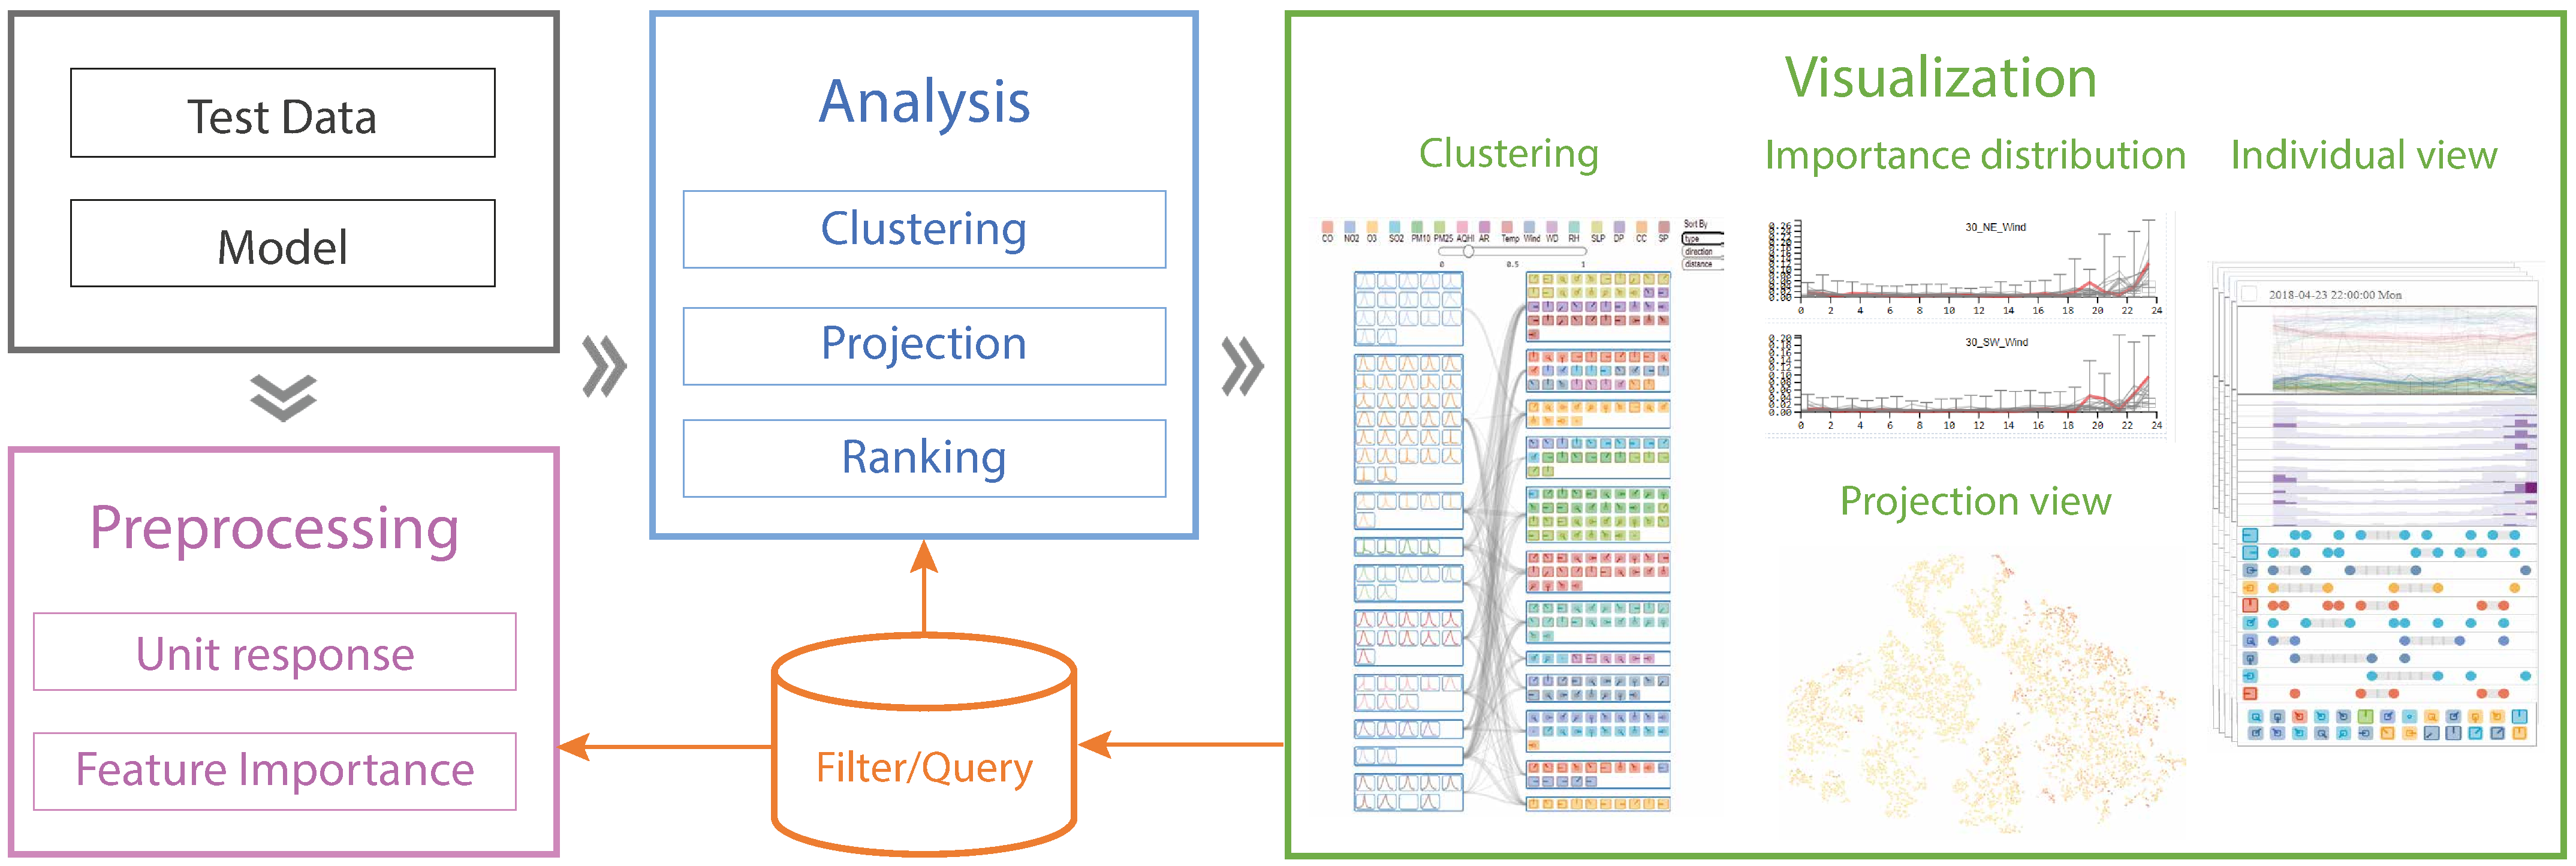
\includegraphics[width=0.49\textwidth]{pictures/System_framework.pdf}
	\vspace{-3mm}
	\caption{The system overview. 
% 	There are three major modules in our system: The preprocessing module estimates the hidden unit response and calculate the feature importance; the analysis module discovers patterns of the model's behaviors; the visualization module provides interfaces for the users to explore the model behavior.
	}
	\label{fig:system_framework}
	\vspace{-4mm}
\end{figure}


We implement MultiRNNExplorer as a web-based system using Flask, VueJS, and D3. 
% \yh{Shall we include model training?}
The system consists of three modules: 1) preprocessing, 2) analysis, and 3) visualization.
% Fig. \ref{fig:system_framework} shows the system framework consisting of three modules including: 1) preprocess, 2) analysis and 3) visualization. 
With chosen models, the preprocessing module is responsible for providing the raw data that need to be analyzed, including extracting hidden states and generating feature importance estimated from the testing data.
% The analysis module run data mining techniques to the extracted information by clustering, projection, ranking.
We then apply various data mining techniques such as clustering, projecting, and ranking in the analysis module to provide the information required by the visualization module.
% The clustering and projection techniques are applied to reveal the model mechanism by \QM{reducing redundant information of the relationship of high-dimension features}, the configurable ranking and mapping are conducted to extract the information of interest. 
The visualization module integrates coordinated views to support interactive interpretation of and reasoning about the model behavior at different perspectives. 
The cluster view summarizes the hidden units' response to features.
The projection view projects the individual cases by using t-SNE, which provides the users an overview of all individual cases.  This view also allows users to find and select cases of interest for further analysis.
The importance distribution view shows the feature importance by timestamps. The ranking of the general importance will be updated according to the selected individual cases.  
The sequence view enables users to explore the data at an individual level including the feature trend, cluster importance and the top features. 
A rich set of interactions are also supported to link different views together.



% In this section, the system overview are discussed as Fig ~\ref{fig:system_framework}. The whole system consists of three components: model manager, model interpreter and visualization. 

% The model manager is designed to manipulate trained models and enable users to select the dataset they are interested in. With a choosing model and dataset, the model manager will manage the input data, output of each hidden states, and the gradient of input with respect to the hidden states output into the files.    

% With the output of model manager, then the model interpreter calculates the distribution of hidden states output first. Then it extracts the correlation graph by analyzing the difference of these distributions. At last, the model interpreter discover the dependency relations between the hidden state through the input gradient which will be discussed in section 5. 

% The distribution, correlation graph and dependency table will be finally provided to the visualization module. The visualization~\ref{fig:teaser} has six components, the control panel enable users to select the test data, trained model and configure parameters. The cluster view visualize the overview relationship between the variables and hidden units, users are allowed to interactively verify if a pattern is captured by the RNN model. The projection view projects the filtered sequence by using tsne which allow users identify how the hidden states are able to \QM{distinguish the different patterns}. The sequence view enable users to explore the data at individual level, where the temporal dependency between each hidden states and the dependency between the hidden states and input data will be visualized. All views are linked when common items are selected. 

